%File: submission_v8.tex --- AAAI-27 anonymous submission (v7-review response: cohort-corrected controls, BH-adjusted coverage inference, MovingAI probe+rescue, claim narrowing)
% "An Empirical Analysis of Transfer for Dynamic Path Planning"
% Built on the official AAAI-27 author kit (aaai2027.sty, TemplateVersion 2027.1).
\documentclass[letterpaper]{article} % DO NOT CHANGE THIS
\usepackage[submission]{aaai2027}  % DO NOT CHANGE THIS
\usepackage[hyphens]{url}  % DO NOT CHANGE THIS
\usepackage{graphicx} % DO NOT CHANGE THIS
\urlstyle{rm} % DO NOT CHANGE THIS
\def\UrlFont{\rm}  % DO NOT CHANGE THIS
\usepackage{natbib}  % DO NOT CHANGE THIS AND DO NOT ADD ANY OPTIONS TO IT
\usepackage{caption} % DO NOT CHANGE THIS AND DO NOT ADD ANY OPTIONS TO IT
\frenchspacing  % DO NOT CHANGE THIS
%
% Recommended for better-looking tables
\usepackage{booktabs}
\usepackage{amsmath}
%
\pdfinfo{
/TemplateVersion (2027.1)
}
\setcounter{secnumdepth}{0}

% Custom macros

\title{An Empirical Analysis of Transfer for Dynamic Path Planning}
\author{
    Anonymous Submission
}
\affiliations{
}

\begin{document}

\maketitle

\begin{abstract}
We study the dynamic path planning problem, where an agent needs to plan a route in the presence of moving obstacles. In particular, we study whether heuristics learned in training maps can be transferred---zero-shot or from a few labeled target maps---to new environments for this task. We show that, with the right training objective and planner integration, a frozen heuristic transfers zero-shot across the procedural continuous dynamic suites---even given no information about future obstacle motion---improving success over a geometric anchor while substantially reducing search effort. Selected discrete-grid experiments show a smaller rank-only effect. With a few labeled target maps, low-rank adaptation preserves the transferred prior while full fine-tuning overtakes it on search effort, at near-parity success, as supervision spans more target worlds---and a matched-label factorial shows that the coverage of distinct target worlds, not raw label count, predicts when full fine-tuning preserves held-out success. Further, across comparable backbones no architecture is uniformly best: Multilayer Perceptrons, Long Short-Term Memory models, Hierarchical Reasoning Models and U-Net architectures all produce useful learned heuristics in different tested formulations, while hierarchy-specific gains do not persist.
\end{abstract}

\section{Introduction}

Dynamic path planning searches over both configuration and time: when obstacles move, a planner must consider waiting, detouring, and timing, and the search space grows accordingly \citep{silver2005cooperative,phillips2011sipp}. The geometric admissible heuristics that make A\textsuperscript{*} \citep{hart1968astar} efficient on static maps ignore exactly these temporal effects, so search effort grows sharply in the presence of moving obstacles. Learned heuristics can reduce search effort \citep{arfaee2011bootstrap,bhardwaj2017sail,yonetani2021neuralastar}, but a deployed planner benefits only if a heuristic trained on one set of maps remains useful on maps it has never seen. We study zero-shot and few-shot transfer of learned heuristics to unseen environments for dynamic path planning; budgeted time-expanded A\textsuperscript{*} serves throughout as a controlled measurement substrate, not a proposed replacement for dedicated dynamic planners.

We organize the experiments around three factors---the training formulation, the way the prediction enters the planner, and the distribution of target supervision---each evaluated first on static suites, where supervision is exact, then under deterministic dynamics. Comparisons use matched controls throughout---twin models differing in one input, identical weights under different integrations, anchor-calibrated budgets, map-level paired inference \citep{henderson2018matters,agarwal2021precipice,pineau2021reproducibility}---and confirmatory comparisons, units, and criteria were specified before test evaluation. Across the tested settings, representation, planner integration, and supervision regime explain the observed transfer outcomes more consistently than model family.

Our contributions are:
\begin{itemize}
    \item \textbf{Dynamic zero-shot transfer with one fixed learned heuristic.} A single U-Net heuristic---development-selected, frozen before the confirmation cohort was generated, and given no future-motion input---improves success on all six dynamic suites of a 50-map-per-suite confirmation cohort ($+0.18$ to $+0.84$; every paired map-level CI excludes zero) and cuts matched search effort by 73--95\%. Three suites are held out: one distinct topology and two parameter/scale shifts; the remaining three are disjoint maps from trained families.
    \item \textbf{Planner integration changes whether transferred predictions reduce search.} Changing the input--target--output formulation rescues a collapsed recurrent model; changing only the planner integration turns an inert discrete residual into useful guidance; and sharing one search state turns an exact oracle from a six-map loss into a six-map win. A negative planning result therefore does not isolate the model unless target and search interface are held fixed.
    \item \textbf{Distinct-world coverage, not label count, predicts adaptation stability in the matched-label factorial.} With scarce static supervision, low-rank adaptation preserves the transferred prior while full fine-tuning is unstable; with more supervision, full fine-tuning often overtakes it on search effort at near-parity success (direct map-paired contrasts at both ends). A matched-label factorial ties the low-supervision failure to concentration in too few distinct worlds, not raw label count: distributing the same labels across more worlds rescues full fine-tuning, and targeted independent world-draw replications preserve the coverage contrasts. Low-rank adaptation shows the least frequent and smallest degradation across the tested cells, though one redraw produces a significant LoRA degradation.
\end{itemize}
Stronger controls delimit the first contribution: success-tuned weighted A\textsuperscript{*} stays grid-robustly behind on spiral and near parity elsewhere at better path quality on two suites, unbudgeted safe-interval planning solves every feasible instance optimally, and the success advantage does not reproduce in a small MovingAI-derived boundary test (diagnosed and repaired below). Boundary experiments: future-window inputs, adapter interpolation, and hierarchy-specific depth add no consistent value; a restricted-observation heuristic with one Bellman backup and frozen scale calibration beats a complete-map comparator on expansions.

\begin{figure*}[t]
\centering
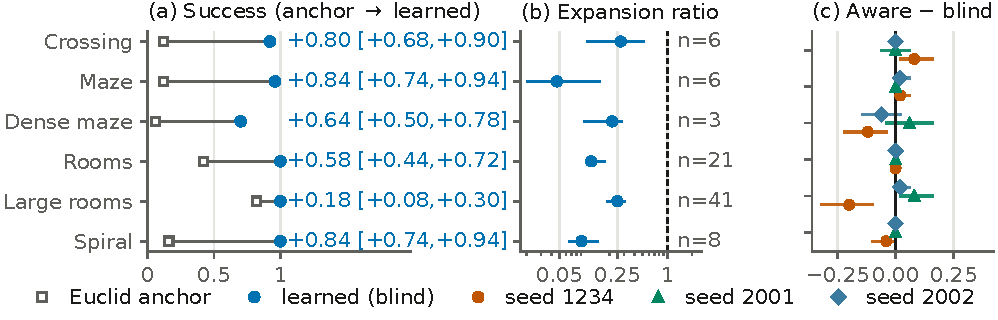
\includegraphics[width=0.98\textwidth]{figures/fig_dynamic_headline.pdf}
\caption{Dynamic zero-shot transfer of one fixed blind U-Net heuristic (blind = no future-motion input) on the 50-map-per-suite confirmation cohort (held-out and trained-family suites as described in the text). (a) Anchor and learned success per suite; labels: paired mean delta with map-level 95\% CI (all six exclude zero; marginal). (b) Matched-solved expansion ratios, conditional on joint success (log axis, map-level 95\% CIs); $n$ = jointly solved count (dense maze $n{=}3$ descriptive). (c) Aware$-$blind success differences for the three training pipelines; the large-rooms cell flips sign.}
\label{fig:dynamic}
\end{figure*}

\section{Problem Formulation and Learned-Heuristic Interfaces}

\textbf{Planning problems.} In the continuous setting, a point robot plans on a probabilistic roadmap \citep[PRM;][]{kavraki1996prm} built over a square world of side length $L{=}1.0$ ($2.0$ for the large-room family); units are abstract. Each roadmap has 192 nodes in total---the start and goal at indices 0 and 1 plus 190 sampled free-space nodes---connected by $k{=}7$ nearest-neighbor candidate edges per node (doubled for the start and goal, then symmetrized into an undirected graph); edges are validated by sampled collision checks at resolution $0.01L$, and unconnected worlds are rejected. Static search states are roadmap nodes, edge costs are Euclidean lengths $\ell(e)$, and the anchor heuristic is Euclidean distance to the goal, $h_0(v) = \lVert x_v - x_g \rVert$. In the dynamic setting, obstacles move on deterministic trajectories and the search state is a pair $(v,t)$ of node and discrete time step of duration $\Delta t$. The planner may traverse an edge, taking $\tau(e) = \lceil \ell(e) / (v_{\mathrm{agent}} \Delta t) \rceil$ steps, or wait one step; transitions are validated against the obstacle trajectories by sampled collision checks along the edge and interval. Cost is arrival time in steps, search runs to a horizon $t_{\max}$, and the anchor is the travel-time lower bound $h_0(v,t) = \lVert x_v - x_g \rVert / (v_{\mathrm{agent}} \Delta t)$, constant in $t$, so anchor and cost share units. In the discrete setting, agents plan on occupancy grids of $20{\times}20$ to $256{\times}256$ cells with Manhattan distance as the anchor.

\textbf{Supervision targets.} With $h^{*}$ the exact cost-to-go (graph Dijkstra on the static roadmap; backward space--time Dijkstra over $(v,t)$ in the dynamic setting), the regression target is the normalized anchor residual $\bar\delta^{*}(s) = \mathrm{clip}\!\left(h^{*}(s) - h_0(s),\, 0,\, c\,T\right)/T$, where $T$ is the normalization scale ($T{=}L$ statically; $T = L/(v_{\mathrm{agent}}\Delta t)$, the map-crossing time in steps, dynamically---the same value for every suite by construction) and the cap is $c{=}4.0$ in normalized units, applied after normalization; unreachable states are masked from the loss. Scalar models predict $\bar\delta_\theta$ from per-node feature tokens; field models predict a goal-conditioned residual raster (eight input channels; appendix) sampled at node positions. At integration the prediction is rescaled: $\hat h_\theta(s) = h_0(s) + T \cdot \mathrm{clip}(\bar\delta_\theta(s), 0, c)$.

\textbf{Planner integrations.} Under \emph{additive} integration the planner orders states by $f(s) = g(s) + \hat h_\theta(s)$, sacrificing admissibility for guidance; empirical path-cost ratios are reported wherever additive integration is used. The classical control is weighted A\textsuperscript{*} \citep{pohl1970}, which orders states by $f(s) = g(s) + w_h\, h_0(s)$ with a per-suite success-tuned inflation $w_h$. Under \emph{focal (rank-only)} integration \citep{pohl1970,pearl1982semiadmissible}, the anchor priority $f_0(s) = g(s) + h_0(s)$ defines the band $\mathrm{FOCAL}_w = \{ s \in \mathrm{OPEN} : f_0(s) \leq w \cdot \min_{u \in \mathrm{OPEN}} f_0(u) \}$, and the learned prediction orders expansions only within the band. At $w{=}1.0$ the learned score merely breaks ties among minimum-priority states, preserving the anchor's path-cost optimality when search completes (finite budgets can still change success). In the restricted-observation study, learned predictions serve as exit values of a radius-bounded local subgraph; one inference-time Bellman backup over that subgraph produces the heuristic, with a scale calibrated once on a disjoint block.

\textbf{Transfer protocol.} Zero-shot transfer applies a trained-and-fixed heuristic to unseen maps and unseen map families with no target supervision. Few-shot adaptation draws $K$ labeled target maps and compares low-rank adaptation \citep[LoRA;][]{hu2021lora} (rank 8 for the HRM, rank 24 for the wider ON-LSTM), full fine-tuning, and training from scratch (LoRA and full fine-tuning start from the same trained checkpoint; scratch uses the same architecture and schedule from random initialization).

\section{Experimental Setup}

\textbf{Environment families.} A \emph{family} is a procedural map generator; a \emph{suite} is a named evaluation condition; a \emph{world} is one sampled environment. Continuous worlds come from our procedural generator (specification tables in the appendix; code in the anonymized artifact archive accompanying the submission). The static hard families are wall constructions---\emph{maze}/\emph{dense maze} (corridor mazes; the dense variant narrows gaps to $0.115L$), \emph{rooms}/\emph{large rooms} (partition walls with doorways; the large variant doubles the side length), \emph{spiral}, and \emph{bugtrap} (exact generator rules in the appendix). Static training uses the maze, rooms, and spiral families; dense maze, bugtrap, and large rooms are held out (bugtrap: distinct topology; dense maze/large rooms: gap- and scale-shifted variants of trained generators). Dynamic suites add 3--5 moving circular obstacles per world that sweep line segments with triangle-wave motion (radius 0.055--0.080$L$, span 0.36--0.50$L$, period 0.14--0.30 of the horizon; per-suite parameters in the appendix), plus a \emph{crossing} open-arena suite as a timing control. \emph{Dynamic training draws worlds only from the dynamic maze, rooms, and spiral families; dynamic dense maze, crossing, and large rooms are held out}---crossing a distinct open-arena topology, dense maze narrower corridors and adjusted patrollers, large rooms doubled scale with a faster agent---so three of six test suites share a generator with training (disjoint maps) and three are suite-level shifts. No learned model observes a test world during training; evaluation cohorts come from disjoint seed ranges, checked by world fingerprints.

\textbf{Models.} Scalar models consume per-node token sequences (62 tokens of 16 dimensions; appendix) and include an MLP, an LSTM \citep{hochreiter1997lstm}, an ON-LSTM \citep{shen2019onlstm} (1{,}252{,}481 parameters), and a Hierarchical Reasoning Model \citep[HRM;][]{wang2025hrm} (2{,}158{,}529 parameters) with an adaptive-computation port \citep{graves2016act,banino2021pondernet}. Field models consume the eight-channel $64{\times}64$ raster and include a FiLM-conditioned U-Net \citep{ronneberger2015unet,perez2018film} (3{,}702{,}370 parameters), a field HRM (4{,}016{,}642), and a field ON-LSTM (1{,}448{,}578); dynamic variants append $W$ future-occupancy channels ($W{=}8$ aware = ground-truth occupancy at offsets $t{+}1,\ldots,t{+}8$; $W{=}0$ blind). Unless a specific experiment states otherwise, the continuous residual models train with AdamW (learning rate $2{\times}10^{-4}$, weight decay $10^{-4}$, batch 256, gradient clipping 1.0) on a smooth-L1 loss over the capped normalized residual; complete architecture and optimizer tables (including the mission experiments' MLP, LSTM, and graph-network configurations) are in the appendix. Within each direct architecture comparison, models are trained under one matched recipe on identical data.

\textbf{Evaluation.} Each suite is evaluated at a per-suite expansion budget selected by anchor-only calibration: the grid budget whose anchor success is closest to pre-specified targets (evenly spaced in $[0.45, 0.70]$; ties smaller) is fixed---the smallest selected budget is binding---before any learned method is compared. The grid is coarse, so realized anchor success can fall outside the target band (0.05--0.75 dynamic at calibration time, 0.25--0.62 across formal static cells; full grid, selections, and realized rates in the appendix). Static calibration shares worlds with evaluation (anchor-only, never touching learned outcomes; disclosed), so we describe those runs as calibrated benchmark evaluations. The dynamic 50-map cohort and the 144-map restricted-observation cohort are \emph{confirmation} cohorts: their budgets were frozen before the cohorts were generated. Success means reaching the goal within the budget; appendix curves up to $4\times$ binding mitigate single-threshold dependence. Search effort is the \emph{matched-solved expansion ratio}: the median over jointly solved maps of the per-map ratio of learned to anchor expansions. Because it conditions on joint success, it can favor methods that solve only easier maps; success is therefore reported first, with path-cost ratios reported separately (appendix).

\textbf{Statistics.} Success comparisons use paired McNemar tests with Benjamini--Hochberg correction within each experiment's suite family (adjusted values reported as $q$). Interval estimates are percentile bootstraps with 10{,}000 resamples; the resampling unit is the evaluation map, and repeated adaptation or model seeds are averaged within maps before resampling; quoted intervals reflect map uncertainty conditional on the evaluated seeds. Per-suite bootstrap intervals (as in Figure~\ref{fig:dynamic}) are marginal; the corrected McNemar tests are primary (full policy in the appendix). Method-versus-method claims use direct map-paired contrasts. Unless noted, continuous experiments use one primary training seed; the dynamic result adds two retrained pipelines.

\section{Dynamic Zero-Shot Transfer}

\textbf{Setting and fixed-model protocol.} The dynamic experiment trains on the dynamic maze, rooms, and spiral families and evaluates on all six dynamic suites---three sharing a training generator (disjoint maps) and three held out as above (dense maze, crossing, large rooms). The training run keeps 53 usable worlds of 72 candidates, 24 per family (usable: builds, roadmap connects, space--time solvable at $t{=}0$); their tensors hold 1{,}129{,}536 node--time slots, 821{,}850 (72.8\%) of them supervised (appendix). The original 20-map-per-suite cohort served as \emph{development} data: based on it, we selected the field U-Net \emph{blind} twin and froze its checkpoint, additive integration, and per-suite budgets; the 50-map-per-suite \emph{confirmation} cohort was then generated from a pre-specified seed range, map-disjoint by fingerprint check, with no further choices. Selection still happened, on development data; the protocol protects only the confirmation cohort. The blind heuristic receives only current-time occupancy channels; the space--time planner and collision checker always use the true deterministic trajectories when validating $(v,t)$ transitions, so the aware/blind ablation changes only the heuristic's input.

\textbf{Confirmation result.} On the confirmation cohort, the fixed blind U-Net raises success on all six suites: deltas $+0.18$ to $+0.84$, with every paired map-level 95\% CI excluding zero (exact McNemar $q \leq 0.0039$ on all six suites, every discordant map favoring the learned heuristic), and matched expansion-ratio medians of 0.047--0.273---a 73--95\% reduction in search effort on jointly solved maps (Figure~\ref{fig:dynamic}; jointly solved counts 3--41 per suite). Empirical path-cost ratios on solved maps stay within per-suite means of 1.008--1.164, and the pattern reproduces the disjoint development cohort's (appendix). Gains on the three held-out suites ($+0.64$/$+0.80$/$+0.18$) establish transfer under topology and parameter/scale shift; the rest, map-level generalization within trained families.

\textbf{Independent retraining robustness.} Two additional full training pipelines with independent seeds---run, we disclose, at a larger world-collection budget (139/149 usable worlds versus 53; appendix), varying seed and data scale together---reproduce the success pattern on the same held-out cohort: across the three pipelines, 17 of 18 pipeline--suite paired CIs exclude zero (deltas $+0.10$ to $+0.88$; the exception is seed 2001's near-ceiling large-rooms cell, anchor 0.82). Effort magnitudes are stable across pipelines on three suites (medians 0.047--0.135) and pipeline-variable on the other three (0.216--0.625), quoted as across-pipeline ranges there; the retrained models are evaluated on the same 50 maps (retraining robustness, not cohort replication).

\textbf{Tuned weighted A\textsuperscript{*} control.} Because the anchor is deliberately simple, we also compare against weighted A\textsuperscript{*} ($w_h h_0$), success-tuned per suite over $w_h \in \{1.1, 1.2, 1.5, 2, 3, 5\}$ on the development cohort (rule frozen in advance: highest success, ties smaller), evaluated once on the confirmation cohort; the control was specified after the learned results were known, tuning touching only development data (appendix). The comparison yields a three-way tradeoff rather than dominance (Table~\ref{tab:wastar-main}). \emph{Success:} no significant difference is detected on five suites---differences of at most one map on four, and the four-map weighted-A\textsuperscript{*} advantage on the open crossing arena is not significant under the paper's exact McNemar policy ($q{=}0.375$)---while the learned heuristic holds the one BH-significant advantage, on spiral ($+0.30$ $[+0.18,+0.42]$; 15/0 discordant maps, $q{=}3.7\times10^{-4}$). \emph{Effort:} learned-to-weighted expansion medians are below parity everywhere, with the marginal 95\% interval excluding parity on four of six suites (0.217--0.728); the crossing and dense-maze intervals include parity, and these intervals are descriptive---the corrected success tests carry the paper's inferential policy. \emph{Path quality:} on jointly solved maps, the additive learned heuristic pays a premium over tuned inflation whose paired 95\% interval excludes zero on crossing (per-map difference $+0.156$ $[+0.116,+0.200]$) and large rooms ($+0.080$ $[+0.058,+0.105]$); the other four suites stay within $\pm 0.005$ with intervals covering zero. Because three suites selected the grid maximum $w_h{=}5$, we also ran a disclosed post-hoc extension ($w_h \in \{7, 10\}$; design frozen before execution): five selections are unchanged---spiral's development success stays 0.80, so its learned advantage is grid-robust---and dense maze's re-selection to $w_h{=}7$ (development 19/20 versus 18/20) changes no confirmation endpoint: success 0.74 versus 0.70 against both the frozen rows and the learned arm (exact $p \geq 0.5$), effort at parity (median 1.40 $[0.91, 1.67]$), path quality within $\pm 0.007$. The original tuning was not grid-limited on any suite. Full per-suite intervals are in the appendix.

\begin{table*}[t]
\centering
\small
\begin{tabular}{lcccccc}
\toprule
Suite & $w_h$ & Success learned & Success WA* & Expansions learned/WA* [95\% CI] & Cost learned & Cost WA* \\
\midrule
Crossing & 1.5 & 0.92 & 1.00 & 0.825 [0.531, 1.167] & 1.164 & 1.008 \\
Maze & 5 & 0.96 & 0.96 & 0.601 [0.440, 0.835] & 1.013 & 1.017 \\
Dense maze & 5 & 0.70 & 0.70 & 0.982 [0.823, 1.089] & 1.008 & 1.006 \\
Rooms & 3 & 1.00 & 0.98 & 0.554 [0.439, 0.798] & 1.019 & 1.015 \\
Large rooms & 1.5 & 1.00 & 0.98 & 0.728 [0.536, 0.966] & 1.083 & 1.003 \\
Spiral & 5 & \textbf{1.00} & 0.70 & 0.217 [0.183, 0.312] & 1.014 & 1.013 \\
\bottomrule
\end{tabular}
\caption{Fixed learned heuristic versus per-suite success-tuned weighted A\textsuperscript{*} (original grid), confirmation cohort at binding budgets. Expansions: median learned-to-weighted ratio on jointly solved maps [map-bootstrap 95\% CI]. Cost: mean arrival over optimal arrival on the same jointly solved maps (paired intervals in text). Bold: the only BH-significant success difference (exact McNemar $q{=}3.7\times10^{-4}$; crossing's four-map gap $q{=}0.375$). A disclosed post-hoc grid extension re-selects $w_h{=}7$ on dense maze but changes no confirmation endpoint (success 0.74 vs.\ 0.70, $p \geq 0.5$; appendix).}
\label{tab:wastar-main}
\end{table*}

\textbf{Unbudgeted SIPP nearly saturates the substrate.} We also implemented discrete-time SIPP \citep{phillips2011sipp} on the identical substrate with the same collision predicates and the anchor heuristic, gated by a hard correctness check: on all 300 confirmation instances, SIPP's earliest arrival exactly equals the space--time optimum. Run unbudgeted, SIPP solves every feasible instance at optimal path quality---per-suite success 0.94--1.00, exactly the substrate's feasibility ceiling---with small expansion counts in its own interval-state unit (medians 80--290; never merged with $(v,t)$ expansions); wall times per map: SIPP 0.9--1.8\,s, learned pipeline 1.18\,s end-to-end (1.02\,s heuristic table + 0.15\,s search), weighted A\textsuperscript{*} 0.23\,s (appendix). The learned contribution is therefore precise: it restructures effort within budgeted time-expanded A\textsuperscript{*}; it does not outperform a dedicated dynamic planner on this deterministic substrate (appendix table).

\textbf{External-geometry boundary.} To test the claim beyond our own generators, six MovingAI maps \citep{sturtevant2012movingai} (three street, three dungeon) were converted to the canonical substrate (64$\times$64 occupancy, rectangle-decomposed obstacles), given the trained maze-family patroller dynamics, and evaluated with the same frozen heuristic under the frozen calibration/tuning protocol; one dungeon map yields no usable instances, so five maps contribute (appendix). The success advantage does not transfer: the learned heuristic never significantly beats the anchor (deltas $-0.08$ on both groups) and loses to tuned weighted A\textsuperscript{*} on dungeon instances ($-0.28$, 0/7 discordant, exact $p{=}0.016$; instance-level, unadjusted, nested in two maps) while expanding more nodes there (matched ratio 2.20 $[1.25, 6.36]$) and paying path-quality premiums with intervals excluding zero on both groups; only the street-map matched-effort advantage over the anchor survives (0.48 $[0.28, 0.64]$). The zero-shot success claim is therefore bounded to the procedural families and their tested shifts. A residual probe and a few-shot rescue (appendix) locate and repair the failure: predicted-vs-true residual correlation falls from 0.73--0.98 in-distribution to 0.24--0.39 on the converted maps with inflate-only over-prediction, and adapting on 2--8 development instances restores success to 0.90--1.00 (dungeon) and classical parity (street)---with single-instance adaptation degrading street success, the factorial's coverage law on external geometry.

\textbf{Future-window inputs provide no consistent benefit.} The primary model is already the blind twin; the twin study quantifies the future-window contrast directly. Aware and blind twins differ in exactly one input: eight channels of ground-truth future occupancy. On the held-out cohort the contrast is suite-dependent in both directions and unstable across pipelines: of 18 contrasts, the paired interval excludes zero in favor of the aware twin in two, the blind twin in two, and neither in fourteen, and those cells fall in different suites for different pipelines---the large-rooms cell flips sign between pipelines; the canonical pipeline also trained on fewer worlds, but the two collection-matched retrains still disagree (Figure~\ref{fig:dynamic}c; appendix). The original 24 suite-by-backbone cells point the same way, and after full fine-tuning at $K{=}16$, eight of nine success differences are non-positive (the ninth includes zero). We report a failure to observe a systematic future-window benefit under deterministic dynamics---not equivalence, and not harm; stochastic motion is untested.

\section{Effects of Supervision Target and Planner Integration}

\textbf{Static family transfer.} On the six calibrated static suites, the transferred field HRM solves 0.75--1.00 of test maps against anchor success of 0.25--0.58, with BH-adjusted $q$ values from below 0.001 to 0.025 on four suites and matched expansion ratios of 0.521--0.850; three of six suites are held out as above, and pooled source-family models improve success on every held-out family before any target labels.

\textbf{Supervised target.} On the calibrated hard static maps, a pooled ON-LSTM scalar residual model raises hard-maze success from 0.525 to 1.000 over the anchor ($q=4.3\times10^{-11}$), while the parameter-matched scalar HRM collapses to a constant prediction at the residual cap and merely matches the baseline (lower learning rates and a soft cap reproduce the collapse). Retaining the HRM while changing input representation, supervised target, and output head to the raster residual field raises hard-maze success from 0.625 to 0.975 ($q=3.4\times10^{-4}$); a later experiment shows a well-trained scalar HRM is also viable (ratios 0.427--0.822). This localizes the failure to the scalar training formulation, though the field intervention changes several coupled components.

\textbf{Planner integration.} The preferred integration differs between the two tested substrates. On continuous roadmaps, additive residuals exploit the gap the Euclidean anchor leaves (the field-HRM ratios above, at empirical path-cost ratios of roughly 1.02--1.14), while rank-only variants stay closer to plain anchor search. On discrete grids the learned signal is demonstrably informative---the pooled residual correlates 0.987--0.994 with the true residual across map sizes---but its magnitude is scale-flat (predicted-to-true mean falls from 0.73 to 0.19 as maps grow), and every additive configuration in the controlled 22-suite run is at or below its matched baseline. We then reuse the \emph{same} trained predictions only to rank expansions inside a $w{=}1.0$ focal band: expansions fall 6--15\% with no observed success regression \citep{chrestien2023rank}---changing only the integration recovered the ordering signal. We interpret the cross-substrate pattern---additive helping against a looser anchor, ranking against a tighter one---as a hypothesis supported by these results; anchor tightness itself is not directly measured.

\textbf{Oracle integration control.} An oracle control removes model-estimation error: the same exact value ranker loses all six development-map comparisons when paired with a fresh certifier search that discards the incumbent's work (141.2 vs.\ 129.7 expansions) and wins all six when sharing one search queue and $g$-state (122.8)---identical values, only search-state reuse changed (a development mechanism test).

\section{Few-Shot Adaptation}

\begin{figure}[t]
\centering
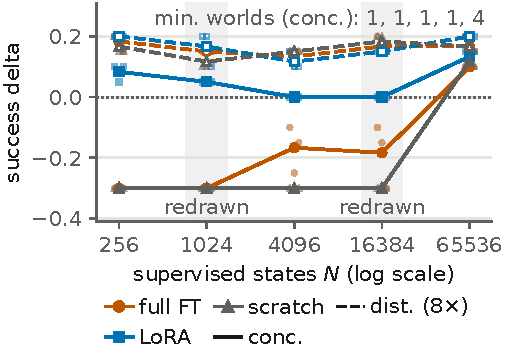
\includegraphics[width=0.98\columnwidth]{figures/fig_c14_dynamic.pdf}
\caption{The matched-label factorial, dynamic substrate (static panel and per-cell tables in the appendix): success delta versus the frozen zero-shot source at fixed supervised-state count $N$, frozen test cohort, binding budgets. Solid: concentrated (fewest worlds supplying $N$; counts annotated); dashed: the same $N$ over $8\times$ as many worlds; small markers: the three adaptation seeds (one sampled world set per cell). Concentrated supervision drops held-out success for full fine-tuning and scratch; distributing the same labels prevents it; recovery at $N{=}65{,}536$ coincides with the world minimum rising to 4. Shaded bands mark $N$ levels with targeted independent world redraws, which preserve positive coverage contrasts there; one redraw LoRA cell degrades (appendix).}
\label{fig:factorial}
\end{figure}

\textbf{Direct contrasts: LoRA protects at $K{=}1$; full fine-tuning overtakes on effort by $K{=}16$.} At $K{=}1$ the map-paired full-FT$-$LoRA success difference is negative in all six target/backbone cells, with the 95\% interval excluding zero in four (worst $-0.600$ $[-0.773,-0.407]$ on large rooms/HRM); LoRA retains the zero-shot gain (dense maze ratio 0.686, success $+0.467$) while full fine-tuning reaches ratio 1.293 on large rooms and scratch is harmful on dense maze ($-0.167$, interval excluding zero). At $K{=}16$ the contrast reverses on effort: the paired expansion-ratio difference favors full fine-tuning in all six cells, with the map-bootstrap interval excluding zero in five (up to $-0.366$ $[-0.489,-0.235]$), at near-parity success (one cell's success interval favors full fine-tuning). A 27-cell matched-compute ablation finds bounded and unbounded LoRA nearly identical (median map-level ratio delta 0.000, maximum 0.037), so the output clamp is not the primary cause of the LoRA plateau; LoRA is not universally protective either (bugtrap ratio 1.153 by $K{=}32$). Dynamic maps are label-dense ($\sim$15{,}507 supervised states per world), and at dynamic $K{=}1$ full fine-tuning is not systematically catastrophic while LoRA continues to improve rather than merely preserve the base. Full per-cell contrasts and illustrative $K$-indexed curves are in the appendix.

\textbf{A matched-label factorial separates label count from distinct-world coverage.} The $K$-indexed protocol confounds two quantities: adding maps adds labels and worlds together. A preregistered factorial therefore holds the number of supervised states $N$ fixed (256 to 65{,}536 by factors of 4) and varies only whether those states are drawn from the fewest worlds that can supply them (\emph{concentrated}) or from eight times as many (\emph{distributed}), in both domains, under matched optimizer steps (Figure~\ref{fig:factorial}; protocol, tables, and regression in the appendix). Each cell adapts one deterministically sampled world set (seeds vary initialization and batch order), with targeted redraws reported separately (appendix). The preregistered primary hypothesis---a full-fine-tuning$\times\log N$ effort crossover---is rejected (interaction $-0.0025$ $[-0.0087, +0.0028]$); the coverage readout below is the prespecified secondary endpoint. Concentrated supervision causes a held-out success drop for full fine-tuning and scratch in both domains---$-0.300$ in every seed at dynamic concentrated $N \leq 1{,}024$, still negative in every seed at $N{=}16{,}384$ from a single world (significantly in one of three)---while distributing the \emph{same} states across more worlds prevents the drop ($+0.15$ to $+0.20$; Figure~\ref{fig:factorial}); direct distributed$-$concentrated contrasts for all 30 cells (appendix) support it under adjusted inference: with BH correction across 30 paired sign-flip tests, the contrast is significant ($q{<}0.05$) for full fine-tuning and scratch in all 10 cells where concentration forces at most two distinct worlds and in none of the 10 where it forces four or more (a threshold identified post hoc, reported descriptively). No significant LoRA success degradation appears in the original 60 cells (worst $-0.067$ $[-0.167, 0.000]$); absent a noninferiority margin this is a failure to observe degradation, not equivalence, and targeted independent world-draw replications at the decisive cells make the caveat concrete: the replicated coverage contrasts are positive in all 18 tested cases---excluding zero for scratch in all six and for full fine-tuning in five of six (the second draw's static contrast touches zero)---but one redraw LoRA cell does degrade, with its interval excluding zero (static concentrated $N{=}256$: $-0.133$ $[-0.267, -0.033]$, still the least-degraded method in that cell; appendix). On the static matched expansion ratios (the domain with adequate jointly solved counts), full fine-tuning is at or below LoRA at every tested $N$ and the full-fine-tuning$\times\log N$ interaction is null ($-0.0025$ $[-0.0087, +0.0028]$); dynamic effort cells contain one jointly solved map and support no inference, and because ratios condition on solved maps, degraded-success cells can look spuriously efficient---so success is the factorial's primary endpoint. The protection low-rank adaptation provides at low supervision appears in \emph{success} and tracks distinct-world coverage rather than label count in this factorial.

\section{Scope and Boundary Results}

\textbf{Discrete transfer.} The pooled HRM base improves mean grid success 0.591$\to$0.612 with lower mean expansions (descriptive); adapters do not improve broadly; a 3--8-seed rank-only pilot on selected maps finds 6--15\% expansion reductions at $w{=}1.0$ with equal or higher observed success (no full-suite confirmation).

\textbf{Architecture and hierarchical depth.} Descriptor-weighted adapter composition routes correctly yet never significantly beats the pooled zero-shot model (appendix) \citep{wortsman2022soups,ilharco2022task}. Architecture rankings differ across tasks and input representations (the U-Net is strongest in the dynamic field study; the HRM holds the lowest single-suite dynamic ratio; the ON-LSTM leads the early calibrated scalar stage). In compositional multi-leg missions with verified oracle headroom (three-seed grids; appendix), no structured model beats the MLP at two depths with a non-decreasing gap, and learned halting moves \emph{opposite} to the depth hypothesis (map-level $\rho{=}-0.578$, permutation $p{=}5\times10^{-5}$); five of 33 recurrent cells suffer constant-prediction collapse and are excluded from capacity conclusions. Follow-ups on persistent memory, iterative refinement, hierarchical substitution, and persistent planning-time search state are also negative (appendix). These are formulation-specific negatives, not claims that recurrence, memory, or hierarchy are universally ineffective \citep{jolicoeur2025trm,czechowski2021subgoal}.

\textbf{Restricted-observation transfer.} Deployed agents rarely observe complete maps, so a final static study restricts the model to a radius-0.20 local subgraph, trains it from behavior-derived returns rather than shortest-path labels, and integrates it through one inference-time Bellman backup over that subgraph. Under a frozen comparison on a disjoint 144-map cohort---whose path-quality gate is the comparator-relative criterion adopted after the original absolute ceiling failed in development (appendix)---this local MLP reduces pooled expansions against the complete-map field HRM by 12.96 (95\% CI $[-16.30,-9.74]$; 109/3/32 wins/ties/losses) at better empirical path quality (cost ratios 1.024/1.162 versus 1.031/1.335), and a separate $w{=}1.10$ bounded control passes all 144 certificates. Sequential ablations locate the sign change at the backup (static insertion loses by $+16$; one backup flips the point estimate to $-1.21$, interval crossing zero; frozen scale calibration then yields the confirmed reduction).
\section{Related Work}

\textbf{Learned guidance for search.} Learned heuristics arise from bootstrapping \citep{arfaee2011bootstrap}, oracle imitation \citep{bhardwaj2017sail}, differentiable search \citep{yonetani2021neuralastar}, grid transformers \citep{kirilenko2023transpath}, classical-planning objectives \citep{ferber2020neural}, and ranking \citep{chrestien2023rank}. We retain classical graph search throughout and jointly evaluate cross-family and dynamic transfer of identical trained models and additive-versus-rank-only integration of the \emph{same} predictions under a shared planner and information set \citep{pohl1970,pearl1982semiadmissible,aine2016mha}.

\textbf{Dynamic, real-time, and motion planning.} The dynamic substrate uses time-expanded space--time search in the spirit of cooperative A\textsuperscript{*} \citep{silver2005cooperative}; safe-interval planning \citep{phillips2011sipp} is a related, faster alternative, which we evaluate as an unbudgeted optimal control. The restricted-observation study relates to real-time heuristic search \citep{korf1990rta,koenig2006rtaa}; its one-step backup resembles a single value-iteration-network update \citep{tamar2016vin,lee2018gppn} and neural algorithm execution \citep{velickovic2021nar}, but runs once, at inference, over a radius-bounded subgraph, to integrate a transferred prediction. Learned samplers and end-to-end motion planners \citep{ichter2018sampling,qureshi2019mpnet} replace the planner itself; we keep a fixed classical planner and learn only its guidance, keeping heuristic transfer measurable on a PRM \citep{kavraki1996prm}.

\textbf{Adaptation and recursive architectures.} LoRA \citep{hu2021lora}, model soups \citep{wortsman2022soups}, and task arithmetic \citep{ilharco2022task} motivate the low-rank and composition studies; the contribution is the low-rank-versus-full-rank comparison as a function of label availability and, through the factorial, supervision distribution across worlds. HRM \citep{wang2025hrm}, adaptive computation \citep{graves2016act,banino2021pondernet}, and simplified recursive models \citep{jolicoeur2025trm} motivate the architecture experiments; our results concern heuristic regression and integration, not their benchmark claims.

\section{Limitations}

\textbf{Design and selection.} Most continuous primary results are single-GPU validations with one primary training seed, and several experiments reuse trained bases or test maps rather than replicating independently. Only the 50-map cohort is selection-free; static calibration shares worlds with evaluation (anchor-only; budget curves mitigate); baselines are the anchor, weighted A\textsuperscript{*}, and SIPP---external \emph{learned} planners are not compared. The retrained pipelines used larger collections (139/149 versus 53 worlds; comparisons vary seed and scale together), and the weighted-A\textsuperscript{*} grid extension was specified post hoc. A suite-indexing defect made the original SIPP, extended-grid, and wall-time runs evaluate sibling cohorts; fingerprint checks exposed it, and all three were re-executed on the frozen cohort under unchanged rules (erratum in the appendix; the weighted-A\textsuperscript{*} baseline used the correct cohort throughout, fingerprint-verified).

\textbf{Statistics and coverage.} The smallest jointly solved cell is three maps; matched-effort magnitudes vary by pipeline on three suites; a best-configuration view in the appendix is post-hoc. Quoted intervals underrepresent training-run uncertainty (addressed dynamically via across-pipeline ranges); the discrete result covers selected cells; map-clustered reanalysis supports the quoted conclusions, though not every exploratory table was regenerated; no equivalence tests were run. The factorial covers one target family per domain, three adaptation seeds, and one sampled world set per cell (targeted redraws in the appendix); coverage counts worlds, not measured geometric diversity; matching covers labels and steps, not world-generation cost; per-cell readouts are marginal (adjusted inference covers the 30 coverage contrasts; the two-world threshold is descriptive). The extended grid and the probe/rescue are post-hoc sensitivity and diagnostic evidence. The primary dynamic experiments report expansions rather than end-to-end latency (timings from a 5-map-per-suite CPU sample; appendix).

\textbf{Scope.} The restricted-observation confirmation is static, one seed and cohort, tests input restriction only (the planner knows the roadmap), carries no formal bound on the direct arm, and is slower in wall time. Dynamic obstacles are deterministic; stochastic motion, kinodynamic constraints, multi-agent coupling, physical robots, and settings beyond 2-D navigation are untested. The external test coarsens and rectangle-decomposes five usable source maps, adds synthetic dynamics, and nests instance-level tests in those maps; SIPP is unbudgeted, its interval unit not resource-equivalent to $(v,t)$ expansions. Negative results are failures to observe improvement under pre-specified protocols, not universal rejections; safety-critical use would need uncertainty-aware motion and collision guarantees.

\section{Conclusion}

A frozen blind U-Net heuristic transferred zero-shot on the procedural substrate: success improved on all six confirmation suites, matched effort fell 73--95\%, and the advantage over success-tuned weighted A\textsuperscript{*} is decisive on spiral, effort-favorable on four suites, and grid-robust. Unbudgeted SIPP solves every feasible instance optimally, and the success advantage does not reproduce on the five MovingAI-derived maps, though a few labeled instances restore it: the contribution is effort structure within budgeted search. Low-rank updates protect under scarce supervision, full fine-tuning overtakes on effort as labels span more worlds, and failure tracks distinct-world coverage, not label count.

\bibliography{references}

% AAAI-27 requires the reproducibility checklist to be uploaded separately
% in the designated submission field; it should not be included in this PDF.

\end{document}
